\chapter{Bucketing}
\label{ch:bucketing}

Bucketing is shmap's substitute for full co-linear chaining (\S\ref{sec:seed-extend}): instead of
clustering individual hits by a general chaining algorithm, the reference is pre-partitioned into
fixed-geometry, \emph{overlapping} windows (\emph{buckets}), and every hit is attributed to the
bucket(s) whose window contains it. This section defines the bucket geometry precisely, then the
two data structures that accumulate hits into buckets (\code{Buckets}, the primary store, and
\code{BucketsHash}, an ephemeral scratch structure), then \code{match\_seeds}, the procedure that
actually populates them from a read's seed list.

\section{Bucket geometry}
\label{sec:bucket-geometry}

Fix a \textbf{half-length} $\ell$ (per read; \S\ref{sec:bucket-halflen}). Bucket slot $b$ (an
integer, possibly negative only in the sense that $b\ge 0$ is enforced but not derived that way
directly) spans the half-open interval
\[
  \bigl[\,b\cdot\ell,\ (b+2)\cdot\ell\,\bigr)
\]
in whichever coordinate space is active (\S\ref{sec:config-axes}: nucleotide position if
\code{abs\_pos}, else index into the segment's sketch array). \textbf{Consecutive buckets overlap
by exactly half their width}: bucket $b$ and bucket $b{+}1$ share the sub-range $[(b{+}1)\ell,
(b{+}2)\ell)$. A position $p$ maps to its \emph{primary} bucket via $b = \lfloor p/\ell \rfloor$;
because of the 50\% overlap, $p$ is \emph{also} inside bucket $b{-}1$ whenever $b>0$ (since bucket
$b{-}1$'s span $[(b{-}1)\ell, (b{+}1)\ell)$ still contains any $p$ with $b\ell \le p <
(b{+}1)\ell$).

\begin{figure}[htbp]
\centering
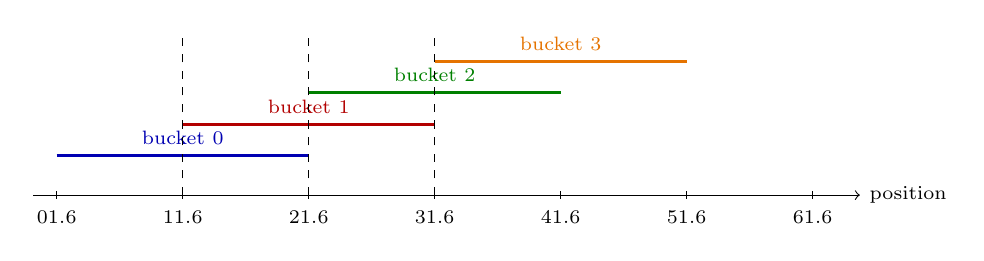
\begin{tikzpicture}[scale=1, every node/.style={font=\scriptsize}]
  \def\ell{1.6}
  \draw[->] (-0.3,0) -- (6*\ell+0.6,0) node[right] {position};
  \foreach \i in {0,...,6} {
    \draw (\i*\ell,0.05) -- (\i*\ell,-0.05);
    \node[below] at (\i*\ell,-0.08) {$\i\ell$};
  }
  \draw[very thick, blue!70!black] (0,0.5) -- (2*\ell,0.5) node[midway,above] {bucket 0};
  \draw[very thick, red!70!black] (1*\ell,0.9) -- (3*\ell,0.9) node[midway,above] {bucket 1};
  \draw[very thick, green!50!black] (2*\ell,1.3) -- (4*\ell,1.3) node[midway,above] {bucket 2};
  \draw[very thick, orange!90!black] (3*\ell,1.7) -- (5*\ell,1.7) node[midway,above] {bucket 3};
  \draw[dashed] (1*\ell,0) -- (1*\ell,2);
  \draw[dashed] (2*\ell,0) -- (2*\ell,2);
  \draw[dashed] (3*\ell,0) -- (3*\ell,2);
\end{tikzpicture}
\caption{Bucket geometry: each bucket spans $2\ell$, consecutive buckets overlap by $\ell$
(50\%). A hit at position $p \in [\ell, 2\ell)$ (e.g.\ the overlap region between buckets 0 and 1)
is attributed to \emph{both} bucket 0 and bucket 1.}
\end{figure}

\paragraph{Why 50\% overlap.} Without overlap, a true alignment straddling a bucket boundary would
have its matches split roughly in half between two non-overlapping buckets, and neither alone
would score well even though the true alignment is real and strong. With 50\% overlap, \emph{any}
true alignment of length up to $\ell$ is guaranteed to be fully contained within at least one
bucket (the one aligned with its start, or its neighbor), at the cost of roughly doubling the
number of (hit, bucket) attributions that must be tracked. This is directly analogous to why
minimizer schemes (\S\ref{sec:minimizers}) guarantee window coverage --- it is the same
``don't let a real signal fall in a seam'' concern, solved geometrically instead of via a
window-based sampling guarantee.

\subsection{Choosing $\ell$: the bucket half-length}
\label{sec:bucket-halflen}

$\ell$ is set once per read, to the read's own sketch size $m$ (or, under \code{abs\_pos}, the
read's raw nucleotide length) --- i.e., \textbf{a bucket is sized to be exactly as wide as the
read it's being used for}, so that a bucket can plausibly contain one full copy of the read's
alignment. A minimum half-length $\ell_{\min}=5$ is enforced as a sanity floor (extremely short
reads/sketches are rejected as unmappable rather than creating degenerate buckets).

\section{\code{Buckets}: the primary per-run accumulator}
\label{sec:buckets-struct}

One \code{Buckets} instance is created once per mapping run (not per read) and \code{clear()}'d
between reads (\S\ref{sec:buckets-clear}) --- this reuses its backing storage rather than
reallocating per read.

\begin{center}
\begin{tabularx}{\textwidth}{@{}llX@{}}
\toprule
\textbf{Field} & \textbf{Type} & \textbf{Meaning} \\
\midrule
\code{halflen} & int & Current read's $\ell$ (\S\ref{sec:bucket-halflen}); reset every read. \\
\code{i} & int & Index of the next seed (into the current read's seed list) not yet propagated to
  every touched bucket's own \code{.i} counter (\S\ref{sec:bucket-propagate}). \\
\code{seeds} & int & Seed-occurrence budget consumed so far, mirrored into every touched bucket. \\
\code{buckets} & one \code{Vec<BucketContent>} per segment & Flat, directly-indexed storage:
  \code{buckets[segm\_id][b]} is that bucket's running \code{BucketContent}
  (\S\ref{sec:type-bucketcontent}), pre-sized to $\lceil \mathit{segment\_length}/\ell_{\min}
  \rceil + 2$ slots at construction time so that it is large enough for \emph{any} valid $\ell \ge
  \ell_{\min}$ used later. \\
\code{non\_empty\_buckets\_with\_repeats} & \code{Vec<BucketLoc>} & Every \code{BucketLoc} touched
  since the last \code{clear()}, \textbf{with duplicates} (a bucket touched by 5 different hits
  appears 5 times) --- deduplicated only when \code{get\_sorted\_buckets} is called
  (\S\ref{sec:get-sorted-buckets}). Doubling as the undo-log for \code{clear()}. \\
\bottomrule
\end{tabularx}
\end{center}

\begin{notebox}
The reference C++ caps the number of reference segments at a hardcoded constant
(\code{MAX\_SEGMENTS = 100}), throwing at construction time for larger references. This reads as
an arbitrary implementation limit, not an intentional one --- draft/scaffolded genome assemblies
routinely have thousands of small contigs. A from-scratch implementation should size
\code{buckets} to the reference's \emph{actual} segment count instead of imposing any fixed cap.
\end{notebox}

\subsection{\code{clear()}}
\label{sec:buckets-clear}

\begin{algobox}{title={\code{Buckets::clear}()}}
\begin{verbatim}
i := 0
seeds := 0
for (segm_id, b) in non_empty_buckets_with_repeats:
    buckets[segm_id][b] := BucketContent::default()   # reset just the touched slots
non_empty_buckets_with_repeats.clear()
\end{verbatim}
\end{algobox}

Only slots that were actually touched are reset (tracked via the repeats log) --- this is
$O(\text{touched slots in the previous read})$, not $O(\text{reference size})$, which matters
because the vast majority of a genome-scale reference's buckets are never touched by any single
read.

\subsection{\code{add\_to\_pos} and \code{add\_to\_bucket}}

\begin{algobox}{title={\code{add\_to\_pos}(hit, content) / \code{add\_to\_bucket}(loc, content)}}
\begin{verbatim}
function add_to_pos(hit, content):
    b := (abs_pos ? hit.r : hit.tpos) / halflen        # integer division
    buckets[hit.segm_id][b] += content                  # BucketContent's additive merge
    log(hit.segm_id, b)
    if b > 0:
        buckets[hit.segm_id][b-1] += content             # 50% overlap: also touches predecessor
        log(hit.segm_id, b-1)

function add_to_bucket(loc, content):
    buckets[loc.segm_id][loc.b] += content
    log(loc.segm_id, loc.b)
\end{verbatim}
\end{algobox}

\code{add\_to\_pos} is the geometry-aware entry point (a raw hit maps to exactly one primary
bucket $b$, plus its overlap-neighbor $b{-}1$, per \S\ref{sec:bucket-geometry}); \code{
add\_to\_bucket} is a direct write to an already-known bucket location, used when the caller has
already done bucket-location arithmetic itself (\S\ref{sec:match-seeds}, for multi-hit seeds).

\subsection{Propagating the seed cursor: \code{propagate\_seeds\_to\_buckets}}
\label{sec:bucket-propagate}

\begin{algobox}{title={\code{propagate\_seeds\_to\_buckets}()}}
\begin{verbatim}
for (segm_id, b) in non_empty_buckets_with_repeats:
    buckets[segm_id][b].i := i
    buckets[segm_id][b].seeds := seeds
\end{verbatim}
\end{algobox}

Called once, after \code{match\_seeds} (\S\ref{sec:match-seeds}) has consumed the full seed
budget $S$ for the read: every touched bucket's own \code{.i}/\code{.seeds} counters are
initialized to the \emph{global} cursor position, so that incremental pruning
(Chapter~\ref{ch:pruning}) can resume extending each bucket from exactly where uniform seed
consumption left off, without having to replay every seed from scratch per bucket.

\subsection{\code{get\_sorted\_buckets}}
\label{sec:get-sorted-buckets}

\begin{algobox}{title={\code{get\_sorted\_buckets}()}}
\begin{verbatim}
sort non_empty_buckets_with_repeats by (segm_id, b)
deduplicate consecutive equal entries
result := [ (loc, buckets[loc.segm_id][loc.b]) for loc in deduplicated ]
sort result by content.matches descending
return result
\end{verbatim}
\end{algobox}

This is the hand-off point to pruning/refinement (Chapters~\ref{ch:pruning}--\ref{ch:scoring}):
buckets are visited \textbf{most-matches-first}, so that the best candidates raise the acceptance
threshold as early as possible, making the seed-heuristic bound (\S\ref{sec:seed-heuristic-theory})
prune later (worse) buckets even more aggressively.

\begin{notebox}
The reference C++ uses \code{std::sort}, whose relative order for \emph{tied} match counts is
unspecified (and not even guaranteed stable across compiler/standard-library versions). A
from-scratch implementation using a stable sort will therefore not, in general, reproduce the
exact tie-broken order the reference binary happens to produce on any given build --- this is a
property of the reference implementation, not a target worth chasing; downstream results only
depend on tie-breaking when two buckets score \emph{exactly} equally, which is rare in practice
and does not affect which bucket is ultimately reported as long as the final selection compares
scores explicitly (which it does, \S\ref{sec:match-rest}).
\end{notebox}

\section{\code{BucketsHash}: ephemeral scratch structure for one multi-hit seed}
\label{sec:buckets-hash}

A second, hash-map-backed structure with the same \code{add\_to\_pos} geometry (keyed by
\code{BucketLoc} directly, rather than a flat per-segment array) is used \emph{only} as short-lived
scratch space, local to processing a single seed with more than one reference hit
(\S\ref{sec:match-seeds}) --- never as an alternative backing store for the main per-run
\code{Buckets}. It needs no \code{clear()}/undo-log machinery since a fresh instance is created
per multi-hit seed and discarded immediately after.

\section{\code{match\_seeds}: populating buckets from the seed budget}
\label{sec:match-seeds}

\paragraph{Input.} The read's sorted seed list (Chapter~\ref{ch:seeding}), the (per-run,
just-cleared) \code{Buckets}, and the seed budget $S$ (occurrences, \S\ref{sec:seed-budget}).

\paragraph{Output.} None (mutates \code{buckets} in place); also returns/accumulates the total
seed-match count for diagnostics.

\begin{algobox}{title={\code{match\_seeds}(seeds, buckets, S)}}
\begin{verbatim}
while buckets.i < len(seeds) and buckets.seeds < S:
    seed := seeds[buckets.i]
    if seed.hits_in_t > 0:
        if seed.hits_in_t == 1:
            hit := index.h2single[seed.kmer.h]
            content := BucketContent(matches=1, seeds=0,
                                      codirection = (hit.strand==seed.kmer.strand) ? +1 : -1,
                                      r_min=hit.r, r_max=hit.r)
            buckets.add_to_pos(hit, content)
        else:
            # De-duplicate this *one* seed's own multiple reference hits into
            # per-bucket contributions *before* merging into the shared
            # Buckets store, so that a seed occurring k times inside one
            # bucket only ever contributes min(k, occs_in_p) matches to it
            # (a seed cannot match "more than itself" in a single bucket).
            scratch := BucketsHash(halflen = buckets.halflen)
            for hit in index.h2multi[seed.kmer.h]:
                c := BucketContent(matches=1, seeds=0,
                                    codirection = (hit.strand==seed.kmer.strand) ? +1 : -1,
                                    r_min=hit.r, r_max=hit.r)
                scratch.add_to_pos(hit, c)
            for (loc, c) in scratch.buckets:
                clamped := BucketContent(matches = min(c.matches, seed.occs_in_p), seeds=0,
                                          codirection=c.codirection,
                                          r_min=c.r_min, r_max=c.r_max)
                buckets.add_to_bucket(loc, clamped)
    buckets.seeds += seed.occs_in_p
    buckets.i += 1
\end{verbatim}
\end{algobox}

\paragraph{Why the extra de-duplication pass for multi-hit seeds.} A seed with, say,
\code{occs\_in\_p}$=2$ (occurs twice in the read) and \code{hits\_in\_t}$=5$ (occurs 5 times in
the reference) could have several of those 5 reference hits fall inside the \emph{same} bucket.
Without capping, that bucket would be credited with up to 5 matches from a seed that only truly
occurs twice in the read --- overcounting. The scratch structure first tallies, per bucket, how
many of this one seed's reference hits land there, then clamps that tally to
\code{occs\_in\_p} before merging into the shared \code{Buckets} store, guaranteeing a single
seed can never contribute more matches to any one bucket than it actually occurs in the read.

\section{Reference C++ implementation}

\begin{lstlisting}[style=cppstyle,caption={\code{match\_seeds} and \code{Buckets::add\_to\_pos}, \texttt{src/shmap.h} \& \texttt{src/buckets.h}}]
void match_seeds(const Seeds &p_unique, BucketsType &B, qpos_t S) {
    for (; B.i < (qpos_t)p_unique.size() && B.seeds < S; B.i++) {
        Seed seed = p_unique[B.i];
        if (seed.hits_in_T > 0) {
            if (seed.hits_in_T == 1) {
                const auto &hit = tidx.h2single.at(seed.kmer.h);
                BucketContent content(1, 0, hit.strand == seed.kmer.strand ? 1 : -1, hit.r, hit.r);
                B.add_to_pos(hit, content);
            } else {
                BucketsHash<abs_pos> b2m(B.halflen);
                for (const auto &hit: tidx.h2multi.at(seed.kmer.h)) {
                    BucketContent content(1, 0, hit.strand == seed.kmer.strand ? 1 : -1, hit.r, hit.r);
                    b2m.add_to_pos(hit, content);
                }
                for (auto it = b2m.buckets.begin(); it != b2m.buckets.end(); ++it) {
                    BucketContent content(min(it->second.matches, seed.occs_in_p), 0,
                                           it->second.codirection, it->second.r_min, it->second.r_max);
                    B.add_to_bucket(it->first, content);
                }
            }
        }
        B.seeds += seed.occs_in_p;
    }
}

void add_to_pos(const Hit& hit, const BucketContent &content) {
    qpos_t b = (abs_pos ? hit.r : hit.tpos) / halflen;
    buckets[hit.segm_id][b] += content;
    non_empty_buckets_with_repeats.push_back(BucketLoc(hit.segm_id, b));
    if (b > 0) {
        buckets[hit.segm_id][b-1] += content;
        non_empty_buckets_with_repeats.push_back(BucketLoc(hit.segm_id, b-1));
    }
}
\end{lstlisting}

\section{Complexity}

Populating buckets from $S$ consumed seed occurrences costs $O(S \cdot \bar d)$, where $\bar d$ is
the average reference-hit count of a consumed seed (bounded by \code{-M} when set,
\S\ref{sec:max-matches}). \code{get\_sorted\_buckets} costs $O(u \log u)$ where $u$ is the number
of distinct buckets touched this read --- typically far smaller than the reference size, since
only buckets that received at least one seed match are ever touched at all.
